\chapter{Pronghorn: Software for Multiscale Analysis}
\label{sec:ph}

The tightly-coupled multiscale and multiphysics nature of \glspl{pbr}, the importance of \gls{3d} unstructured meshing capabilities, and the restrictive emphasis of earlier modeling tools on gas coolants motivates the development of a new modeling tool in this research to enable application of the models described in Chapter \ref{sec:PhysicalModels} to multiscale analysis of single-phase \glspl{pbr}. This new application, Pronghorn, is a multi-dimensional, coarse-mesh, reactor analysis tool intended to accelerate the design and analysis cycle for \glspl{pbr} with computing requirements within reach of industry and regulatory stakeholders. 

Multiscale analysis at its core is a form of multiphysics analysis\mdash a set of models are coupled together to account for physics feedback effects between various length scales. The key functional requirements in the development of new \gls{pbr} multiscale simulation capabilities are 1)~tightly-coupled solution and data transfer schemes between multiple physics and length scales relevant to nuclear reactors, 2)~efficient simulation on unstructured meshes, and 3)~flexible source code modification to include closures for non-gas coolants. Additionally, new capabilities should be developed with the goal of enhancing modeling tools available to the nuclear engineering community and designed with reuse and longevity in mind.

Many commercial \gls{cfd} applications such as COMSOL and FLUENT include porous media models for fluid flow on unstructured meshes with capacity for user-defined closures and native multiphysics coupling with other physics domains \cite{comsol_cfd,fluent}. However, neutron transport physics, perhaps the most important feedback effect on \gls{th} physics, are often not available in these commercial applications due to export control regulations. While most commercial \gls{cfd} tools include a model builder for implementation of user-defined \glspl{pde}, individual efforts in this area are difficult to reuse across multiple research groups and institutions and often require custom-built testing systems to ensure high software quality. For example, a number of research groups have separately implemented deterministic neutron transport models into local COMSOL license checkouts, duplicating many person-hours of effort that could have been avoided through the use of existing neutron transport solvers \cite{xin_wang,hurt,chandler,xoubi,fiorina}. The heavy use of empirical models for fission gas buildup and irradiation-induced microstructural changes in nuclear materials modeling makes implementation of this second important physics domain in commercial \gls{cfd} tools an additional challenge to comprehensive multiphysics analysis for \glspl{pbr}. Difficulty parallelizing user-defined functions has in some cases restricted these types of software development to serial implementations \cite{becker}.

Commercial applications are also usually closed source, complicating or precluding the adjustment of the numerical solution procedure or physics model. For instance, implementation of acceleration methods to achieve robust numerical performance for neutron transport simulations of a wide range of nuclear systems \cite{willert} may be challenging. The closed source nature of commercial tools is likely a primary motivation for the previously-cited researchers resorting to implementation of deterministic transport models in COMSOL as opposed to coupling an existing tool to COMSOL. The combination of license costs in the thousands to tens of thousands of dollars range, closed source code, and difficulty distributing new physics capabilities within the nuclear engineering community prompt alternative strategies for numerical implementation of the models in Chapter \ref{sec:PhysicalModels}.

Within the nuclear engineering field, several non-commercial tools exist for modeling \gls{pbr} \gls{th}. Examples of these tools include the German Forschungszentrum J{\"u}lich Research Centre THERMIX application, widely used in the design and analysis of \glspl{pbr} in Germany and South Africa \cite{gao,tecdoc1163,THERMIX, zwaan}; the University of Michigan and \gls{nrc} \gls{agree} application frequently applied to prismatic gas reactor analysis \cite{seker}; the \gls{kaeri} GAMMA application \cite{lim}; the Rensselaer Polytechnic Institute \gls{pebfd} application \cite{y_li}; and the Iranian Sharif University of Technology \gls{thpp} application \cite{nouri}.

A significant limitation of many of these tools is the use of structured meshes that are frequently also restricted to \gls{2d} $r$-$z$ geometries. Unstructured meshes are necessary for representing the diverging and converging cones common to many \gls{pbr} beds, while \gls{3d} geometries are needed to capture asymmetric power profiles, \glspl{bc}, and transients such as control rod ejection. THERMIX and \gls{thpp} only include a friction-dominated model, and may not be capable of accurately simulating plena or high-Reynolds number flows. Several applications are also restricted to the ideal gas \gls{eos} for fluid properties, preventing simulation of salt-cooled systems. 

While modifying one or more of these tools to solve the multiscale models in Chapter \ref{sec:PhysicalModels} on a \gls{3d} unstructured mesh is certainly an option, the age of many of the applications may make source code changes and maintenance challenging. Further, modification of one of these tools does not directly address the objective of tightly-coupled solution and data transfer with other physics domains relevant to \glspl{pbr}. For these reasons, development of a new application, Pronghorn, on an existing and modern multi-application computing framework is the best approach to meet the key design objectives of tightly-coupled multiphysics, unstructured meshing, and source flexibility. For reasons to follow, the \gls{moose} framework is selected as the base computing platform for the present work.

\gls{moose} is an open source, distributed- and shared-memory parallel, \texttt{C++} \gls{fe} framework developed by \gls{inl} that enables tightly-coupled implicit solution of nonlinear equations \cite{gaston,moose}. \gls{moose} enables practitioners familiar with the applied math aspects of their application areas to translate those concepts into portable, extensible, and high performance software in a method similar to other general purpose toolkits such as deal.II \cite{dealII91} and OpenFOAM \cite{openfoam}. The \gls{moose} framework combines the LibMesh \gls{fe} library \cite{libMeshPaper} with the nonlinear solution and preconditioning capabilities of the \gls{petsc} together in a modular structure to allow rapid production of new simulation tools. 

The use of a \gls{fe} spatial discretization permits the use of unstructured meshes based on a wide variety of element types, and the \gls{parmetis} library provides \gls{mpi}-based mesh partitioning, while LibMesh provides \gls{amr}. \gls{moose} simulations have demonstrated scalability to over 30,000 cores \cite{kong}. Nonlinear solution is based on the \gls{jfnk} method with Jacobians that can optionally be calculated by \gls{ad} to greatly reduce application development time and improve numerical convergence. 

A simulation tool built on the \gls{moose} framework is referred to as an ``application.'' The hierarchical design and common class inheritance permit in-memory multiphysics coupling of these applications to enable prediction of complex interacting phenomena. Fig. \ref{fig:moose_apps} shows a hierarchical depiction of all of the applications tracked by \gls{moose}'s \gls{ci} system and their relationships to one another \cite{moose_training}. Text within rectangular boxes are the names of \gls{moose} applications, while an arrow pointing from box \(A\) to box \(B\) indicates that application \(A\) depends upon, or ``consumes'' application \(B\). The applications shown in the boxes are a mix of physics modules and fluid property implementations. All applications depend upon the \gls{moose} framework, which consists of the framework and open source physics modules listed at the bottom of the \gls{moose}-labeled rectangle.

\begin{figure}[!h]
  \centering
  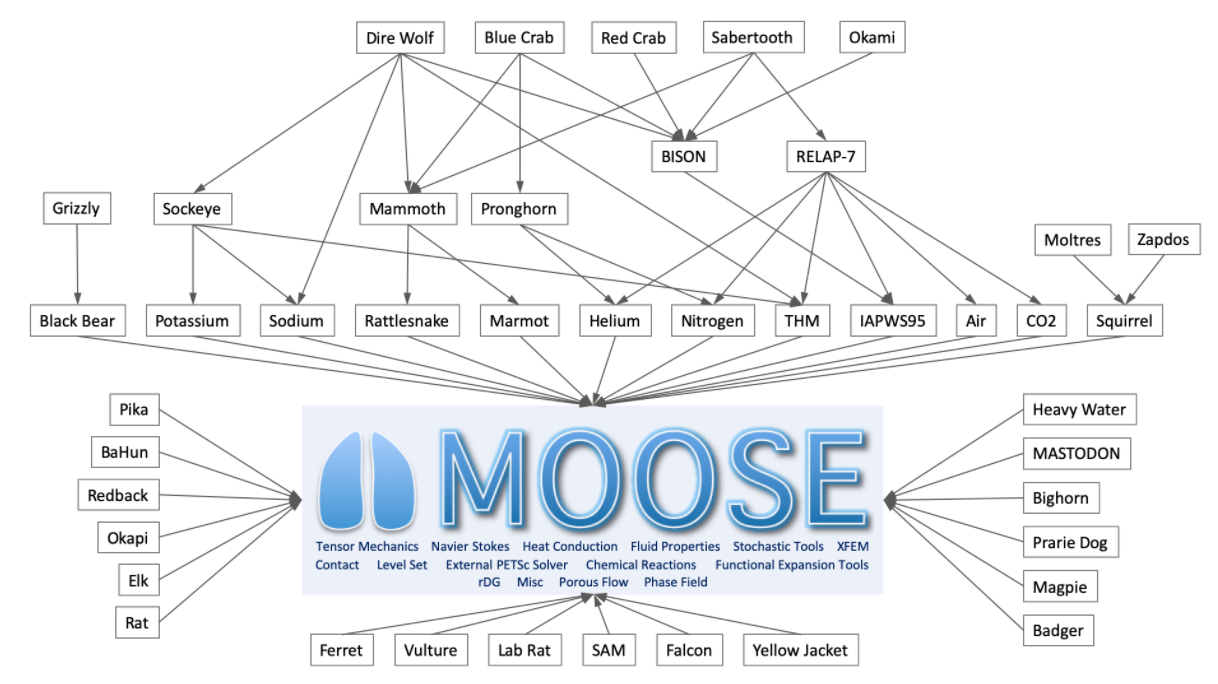
\includegraphics[width=0.9\linewidth]{figs/moose_apps.png}
  \caption{Hierarchical summary of all applications tracked by \gls{moose}'s \gls{ci} system and their relationships to one another \cite{moose_training}.}
\label{fig:moose_apps}
\end{figure}

Examples of applications in the nuclear engineering space include Rattlesnake neutron transport \cite{rattlesnake}; BISON nuclear fuels performance \cite{bison}; RELAP-7 and SAM systems-level \gls{th} \cite{relap7,hu}; and MARMOT phase field \cite{tonks}. The flexible multi-application data transfer and communication design also permits wrapping of external applications by selectively overriding LibMesh \gls{fe} routines to call external libraries. Examples of external wrappings include OpenMC Monte Carlo particle transport and Nek5000 spectral element \gls{cfd} with an application named Okapi \cite{romano, NEK5000, novak}. The \gls{moose} framework also contains a number of open source modules available to all applications, such as a common set of fluid properties and functional expansion data transfer capabilities \cite{wendt}. 

The open source nature of the framework, large user and developer community in areas relevant to \gls{pbr} analysis, native capability for in-memory multiphysics simulations with both peer \gls{moose} applications and external wrapped tools, modular software design, and use of state-of-the-art \gls{3d} unstructured mesh \gls{fe} and solver libraries all contribute to \gls{moose} being the ideal framework upon which to build the next-generation \gls{pbr} \gls{th} solver. As part of this research, the Pronghorn application was developed from scratch to capitalize on the latest advancements in the \gls{moose} framework and its supporting libraries. The remainder of this chapter describes the numerical methods employed for discretization and solution of the models described in Chapter \ref{sec:PhysicalModels}. Section \ref{sec:fem} describes the \gls{fe} spatial discretization and \gls{mol} time discretization. Section \ref{sec:solution} discusses the Picard iteration of multiple applications and nonlinear solution with Newton-Krylov methods. Section \ref{sec:software} then concludes with a brief discussion of the software engineering design.

Throughout this discussion, several brief examples of \texttt{C++} source code are shown to highlight the modular nature and ease-of-development to encourage other applied math practitioners to consider the \gls{moose} framework for their applications. 

\section{Finite Element Discretization}
\label{sec:fem}

This section discusses the discretization of the multiscale models described in Chapter \ref{sec:PhysicalModels} with the continuous \gls{fem}. A comprehensive description of the \gls{fem} is beyond the present scope, and many other texts provide excellent coverage of the method \cite{zienkiewicz,reddy,logan}. 

The objective of this section is to introduce the salient aspects of the method with regards to work performed in this dissertation\mdash that is, implementation of the multiscale models in Chapter \ref{sec:PhysicalModels} within a \gls{fe} framework. Following a high-level discussion of the \gls{fem}, Section \ref{sec:weak_form} presents the weak forms of the governing equations, Section \ref{sec:basis} describes the selection of basis and weight functions, and Section \ref{sec:mol} describes the time discretization. 

The \gls{fem} is characterized by an elegant software implementation and computational efficiency that make it the method of choice for many physics applications, especially for systems with symmetric operators that take advantage of the \gls{fem}'s best approximation properties for self-adjoint differential equations \cite{reddy,zohdi,zienkiewicz}. Unfortunately, the \gls{fem} is conditionally unstable for advection-diffusion equations such as those in Eqs.\ \eqref{eq:PorousEquations} and \eqref{eq:PrimitiveEqns}. Section \ref{sec:supg} therefore concludes this section with a description of a stabilization method implemented to address this shortcoming.

The \gls{fem} is an element-wise application of a Galerkin weighted residual method. Weighted residual methods seek an approximate solution to a differential equation with the assumed form

\beq
\label{eq:WRExpansion}
u=\sum_{j\ =\ 1}^NC_j\phi_j\ ,
\eeq

\noindent where \(u\) is the approximate solution, \(C_j\) are scalar coefficients, \(\phi_j\) are shape functions, and \(N\) is the number of terms in the summation. The discussion in this section is presented in terms of a generic differential equation

\beq
\label{eq:linear1}
K(u_*)=f\ ,
\eeq

\noindent where \(K\) is a nonlinear operator that acts on the true solution \(u_*\) and \(f\) is a function that does not contain \(u_*\). In general, the approximate solution in Eq.\ \eqref{eq:WRExpansion} will not equal the true solution \(u_*\) such that the residual \(R\) is nonzero,

\beq
\label{eq:residual}
R(u)\equiv K(u)-f\ .
\eeq

\noindent Weighted residual methods seek the coefficients \(C_j\) in Eq.\ \eqref{eq:WRExpansion} that minimize the residual with respect to a particular norm. All weighted residual methods can be written in the form

\beq
\label{eq:WR}
\int_\Omega R^*\psi\ d\Omega=0\ ,
\eeq

\noindent where a \(*\) superscript indicates the Hermitian complex conjugate, \(\Omega\) is the phase space, and \(\psi\) is a weight function, also referred to as a ``test'' function. The choice of norm in which to minimize the residual determines the particular form of \(\psi\). The Galerkin weighted residual method chooses \(\psi\) in an attempt to minimize the error \(e\), defined as

\beq
\label{eq:error123}
e\equiv u_*-u\ .
\eeq

\noindent The error is minimized when \(e\) is orthogonal to \(u\), or

\beq
\label{eq:GalerkinErrorMin}
\int_{\Omega}e^*u\ d\Omega=0\ .
\eeq

\noindent The error is in general unknown because the true solution is in general unknown. However, a good approximation of the error is the residual, since the residual is zero when the error is zero. Substituting the residual for the error in Eq.\ \eqref{eq:GalerkinErrorMin}, the Galerkin weighted residual method seeks a solution that minimizes the residual by requiring that it be orthogonal to the approximate solution,

\beq
\label{eq:GalerkinInt}
\int_{\Omega}R^*u\ d\Omega=0\ .
\eeq

\noindent Comparing Eqs.\ \eqref{eq:WR} and \eqref{eq:GalerkinInt}, it is seen that the weight function must lie in the same space as the approximate solution with the exception of the trivial solution. Therefore, \(\psi\) may be expressed in the same basis as \(u\) in Eq.\ \eqref{eq:WRExpansion},

\beq
\label{eq:PsiExpansion}
\psi=\sum_{i\ =\ 1}^ND_i\phi_i\ ,
\eeq

\noindent where different scalar coefficients \(D_i\) are used for generality and to contrast with \(C_j\) in Eq. \eqref{eq:WRExpansion}. More specifically, a Galerkin method with the approximate solution and weight function sharing the same function space is referred to as a Bubnov-Galerkin method. Writing Eq.\ \eqref{eq:GalerkinInt} with \(u\) given by Eq.\ \eqref{eq:WRExpansion} and \(\psi\) given by Eq.\ \eqref{eq:PsiExpansion} gives

\beq
\label{eq:GalerkinInt2}
\bigintsss_{\Omega}\left\lbrack R\left(\sum_{\ j\ =\ 1}^NC_j\phi_j\right)\right\rbrack^*\sum_{i\ =\ 1}^N\phi_i\ d\Omega=0\ ,
\eeq

\noindent where \(R(u)\) indicates that the residual \(R\) may be a general nonlinear function of \(u\). Requiring Eq.\ \eqref{eq:GalerkinInt2} to hold for all \(j\in N\) results in \(N\) equations for the \(N\) coefficients in \(u\),

\beq
\label{eq:GalerkinInt3}
\int_{\Omega}\left\lbrack R\left(C_j\phi_j\right)\right\rbrack^*\phi_i\ d\Omega=0\hspace{1cm}\text{for }j\in N\ .
\eeq

\subsection{The Weak Form}
\label{sec:weak_form}

To ensure a finite integral in Eq.\ \eqref{eq:GalerkinInt3}, the shape functions must be sufficiently differentiable. Define the Hilbert-space norm in \gls{1d} for a function \(\chi\) as

\beq
\label{eq:HilbertNorm}
\|\chi\|_{H^l(\Omega)}\equiv\left\lbrack\sum_{\ j\ =\ 0\ }^{l}\int_{\Omega}\frac{\partial^j\chi}{\partial x^j}\frac{\partial^j\chi}{\partial x^j}d\Omega\right\rbrack^{1/l}\ ,
\eeq

\noindent where \(l>0\) is an integer. For a weighted residual statement with highest derivative \(l\) on the shape functions, finite integrals require that the \(H^l(\Omega)\) norm be finite, or that \(u\in H^l(\Omega)\) and \(\psi\in H^l(\Omega)\). If the residual \(R\) contains higher than first-order derivatives in \(u\), differentiability requirements of the shape functions can be reduced by integrating the residual by parts to transfer some differentiability requirements to the weight function. The resulting equation is referred to as the ``weak form'' of the original ``strong form'' equation. Provided the weak form holds for all choices of \(\psi\), the weak form is equivalent to Eq.\ \eqref{eq:GalerkinInt3} and is solved in this work in place of Eq.\ \eqref{eq:GalerkinInt3}.

The weak form of the Navier-Stokes model is obtained multiplying Eq.\ \eqref{eq:PorousEquations} by \(\psi\) and integrating by parts where possible, giving
\begin{subequations}
\label{eq:PronghornEquations_V2WeakForm}
\begin{align}
\label{eq:MassWeak}
\begin{split}
\int_{\Omega}\epsilon\frac{\partial\rho_f}{\partial t}\psi d\Omega-\int_\Omega\epsilon\rho_f\vec{V}\cdot\nabla\psi d\Omega+\int_\Gamma\epsilon\rho_f\vec{V}\cdot\hat{n}\psi d\Gamma=0&\ ,\\
&\end{split}\\
%
%
\label{eq:MomWeak}
\begin{split}\int_\Omega\left\lbrack\epsilon\frac{\partial(\rho_fV_i)}{\partial t}-\epsilon\rho_f g_i+W\rho_fV_i-P\frac{\partial\epsilon}{\partial x_i}\right\rbrack\psi d\Omega -\int_\Omega \epsilon\rho_fV_i\vec{V}\cdot\nabla\psi d\Omega\ +\hspace{1cm}&\\
\int_\Omega \left(-\epsilon P\frac{\partial\psi}{\partial x_i}+\tilde{\mu}\nabla V_i\cdot\nabla\psi\right)d\Omega+\int_\Gamma\left(\epsilon\rho_fV_i\vec{V}\cdot\hat{n} + \epsilon Pn_i-\tilde{\mu}\nabla V_i\cdot\hat{n}\right)\psi d\Gamma=0&\ ,\\
&
\end{split}\\
%
%
\label{eq:EnergyWeak}
\begin{split}
\int_\Omega\left\lbrack\epsilon\frac{\partial(\rho_fE_f)}{\partial t}-\epsilon\rho_f\vec{g}\cdot\vec{V}+\alpha(T_f-T_s)-\dot{q}_f\right\rbrack\psi d\Omega\ -\int_\Omega \epsilon H_f\rho_f\vec{V}\cdot\nabla\psi d\Omega\ +\hspace{1cm}&\\
\int_\Omega\kappa_f\nabla T_f\cdot\nabla\psi d\Omega+\int_\Gamma\left(\epsilon H_f\rho_f\vec{V}\cdot\hat{n}-\kappa_f\nabla T_f\cdot\hat{n}\right)\psi d\Gamma=0&\ ,\\
&
\end{split}\\
%
%
\begin{split}\int_\Omega\left\lbrack(1-\epsilon)\rho_sC_{p,s}\frac{\partial T_s}{\partial t}+\alpha(T_s-T_f)-\dot{q}_s\right\rbrack\psi d\Omega\ +\hspace{1cm}\\
\int_\Omega\kappa_s\nabla T_s\cdot\nabla\psi d\Omega-\int_\Gamma\kappa_s\nabla T_s\cdot\hat{n}\psi d\Gamma=0&\ .\end{split}
\end{align}
\end{subequations}

\noindent Similarly, the weak form of the friction-dominated model in Eq.\ \eqref{eq:PrimitiveEqns} is
\begin{subequations}
\label{eq:PrimitiveWeakForms}
\begin{align}
\label{eq:Mass2Weak}
\begin{split}
\int_\Omega\epsilon\frac{\partial\rho_f}{\partial t}\psi d\Omega-\int_\Omega\left\lbrack\frac{\epsilon^2}{W}\left(\rho_f\vec{g}-\nabla P\right)\right\rbrack\cdot\nabla\psi d\Omega+\int_\Gamma\left\lbrack\frac{\epsilon^2}{W}\left(\rho_f\vec{g}-\nabla P\right)\right\rbrack \psi d\Gamma=0&\ ,\\
&
\end{split}\\
%
%
\label{eq:Mom2Weak}
\begin{split}\int_\Omega\left\lbrack-\epsilon\rho_f g_i+W\rho_fV_i-P\frac{\partial\epsilon}{\partial x_i}\right\rbrack\psi d\Omega\ -\int_\Omega \epsilon P\frac{\partial\psi}{\partial x_i}d\Omega+\int_\Gamma\epsilon Pn_i\psi d\Gamma=0&\ ,\\
&
\end{split}\\
%
%
\label{eq:Energy2Weak}
\begin{split}
\int_\Omega\left\lbrack\epsilon\rho_fC_{p,f}\frac{\partial T_f}{\partial t}+\epsilon\rho_fC_{p,f}\vec{V}\cdot\nabla T_f+\alpha(T_f-T_s)-\dot{q}_f\right\rbrack\psi d\Omega\ +\hspace{1cm}\\
\int_\Omega\kappa_f\nabla T_f\cdot\nabla \psi d\Omega-\int_\Gamma\kappa_f\nabla T_f\cdot\hat{n}\psi d\Gamma=0&\ ,\\
&
\end{split}\\
%
%
\label{eq:PrimitiveEnergyWeak}
\begin{split}\int_\Omega\left\lbrack(1-\epsilon)\rho_sC_{p,s}\frac{\partial T_s}{\partial t}+\alpha(T_s-T_f)-\dot{q}_s\right\rbrack\psi d\Omega\ +\hspace{1cm}\\
\int_\Omega\kappa_s\nabla T_s\cdot\nabla\psi d\Omega-\int_\Gamma\kappa_s\nabla T_s\cdot\hat{n}\psi d\Gamma=0&\ .\end{split}
\end{align}
\end{subequations}

\noindent In Eqs.\ \eqref{eq:MomWeak} and \eqref{eq:Mom2Weak}, \(i=1,2,3\) represents each component of the momentum equation. The pressure kernel with strong form \(\epsilon\nabla P\) is first written as \(\nabla(\epsilon P)-P\nabla\epsilon\); then, the \(\nabla(\epsilon P)\) term is integrated by parts so that pressure appears in a boundary integral to provide a natural pressure \gls{bc}. 

Finally, the weak form of the meso and micro scale models in Eqs.\ \eqref{eq:oem}, \eqref{eq:MesoscaleSolution}, and \eqref{eq:MicroscaleSolution} is

\beq
\label{eq:MultiscaleWeak}
\int_\Omega\left\lbrack\rho_\jmath C_{p,\jmath}\frac{\partial T_\jmath}{\partial t}\psi+k_\jmath\nabla T_\jmath\cdot\nabla\psi+Q\psi\right\rbrack d\Omega-\int_\Gamma k_\jmath\nabla T_\jmath\cdot\hat{n}\psi d\Gamma=0\ ,
\eeq

\noindent where \(\jmath=S\) and \(Q=\dot{q}_s\) for Eq.\ \eqref{eq:oem}; \(\jmath=\text{meso}\) and \(Q=\la\dot{q}\ra\) for Eq.\ \eqref{eq:MesoscaleSolution}; and \(\jmath=\text{micro}\) and \(Q=\hat{\dot{q}}\) for Eq.\ \eqref{eq:MicroscaleSolution}.

The \gls{moose} framework is designed based on object-oriented programming principles that abstract much of the numerical implementation of Eqs.\ \eqref{eq:PronghornEquations_V2WeakForm}--\eqref{eq:MultiscaleWeak} from the software developer, such as numeric integration, physical-to-master mappings, and looping over the basis and weight function summations in Eqs.\ \eqref{eq:WRExpansion} and \eqref{eq:PsiExpansion}, to \gls{moose} framework classes and the LibMesh \gls{fe} library. Application developers simply need to override the quadrature point residual calculation of base \texttt{Kernel} and \texttt{BoundaryCondition} classes to represent their desired physics. For example, the source code responsible for residual calculation of the diffusive kernel contribution to Eqs.\ \eqref{eq:EnergyWeak} and \eqref{eq:Energy2Weak} at a quadrature point is shown in Listing \ref{lst:one}.

\vspace{1em}
\begin{minipage}[c]{0.92\linewidth}
\begin{lstlisting}[caption={Pronghorn source code calculation of \(\int_\Omega\kappa_f\nabla T_f\cdot\nabla\psi d\Omega\).},captionpos=b,label={lst:one}]
Real
FluidEnergyDiffusiveFlux::computeQpResidual()
{
  return _kappa_f[_qp] * _grad_T_fluid[_qp] * _grad_test[_i][_qp];
}
\end{lstlisting}
\end{minipage}

\texttt{FluidEnergyDiffusiveFlux} is the kernel class name and \texttt{computeQpResidual} is the name of the base \texttt{Kernel} method that provides the residual calculation at a quadrature point. \texttt{\_kappa\_f} is the name of the \(\kappa_f\) material property coupled to the kernel; \texttt{\_grad\_T\_fluid} is the name of the gradient of the fluid temperature \(\nabla T_f\) coupled to the kernel; and \texttt{\_grad\_test} is the name of the gradient of the weight function \(\nabla\psi\), indexed by \texttt{\_i} as shown in Eq.\ \eqref{eq:PsiExpansion}. The base \texttt{Kernel} class loops over the \texttt{computeQpResidual} method at each quadrature point, with index \texttt{\_qp}, to construct the discretized residual.

Each of the kernels and \glspl{bc} in Eqs.\ \eqref{eq:PronghornEquations_V2WeakForm}--\eqref{eq:MultiscaleWeak} are implemented in this manner in Pronghorn. Intermediate \texttt{Material} classes express all possible solution variables\mdash \(P\) and \(\rho_f\) for the mass equation; \(\vec{V}\), \(\vec{v}\), \(\rho_f\vec{V}\), and \(\rho_f\vec{v}\) for the momentum equations; \(T_f\) and \(\rho_fE_f\) for the fluid energy equation; and \(T_s\) for the solid energy equation\mdash as material properties. This enables a flexible coupling in the class constructors that is agnostic to the underlying set of solution variables. Unless otherwise noted, all integrals are evaluated with Gaussian quadrature rules in this work.

The multiscale closures are implemented by overriding the property evaluation of base \texttt{Material} classes. For example, the source code responsible for calculation of the effective fluid thermal conductivity \(\kappa_f\) at a quadrature point is shown in Listing \ref{lst:two}.

\vspace{1em}
\begin{minipage}[c]{0.92\linewidth}
\begin{lstlisting}[caption={Pronghorn source code evaluation of \(\kappa_f\) by Eq.\ \eqref{eq:LinearPecletKappaFluid}.}, captionpos=b,label={lst:two}]
void
LinearPecletKappaFluid::computeQpProperties()
{
  _kappa_f[_qp] = _k_f[_qp] * (_epsilon[_qp] + _C0 * _Pe[_qp]);
}
\end{lstlisting}
\end{minipage}

\texttt{LinearPecletKappaFluid} is the material class name corresponding to the closure in Eq.\ \eqref{eq:LinearPecletKappaFluid} and \texttt{computeQpProperties} is the name of the base \texttt{Material} method that provides the material property calculation at a quadrature point. \texttt{\_kappa\_f} is the name of the computed property. \texttt{\_epsilon}, \texttt{\_k\_f}, and \texttt{\_Pe} are the names of the porosity \(\epsilon\), fluid thermal conductivity \(k_f\), and Peclet number \(Pe\), materials coupled to the \texttt{LinearPecletKappaFluid} material, respectively. \texttt{\_C0} is the name of a user-specified scaling parameter. Each of the closures in Eqs.\ \eqref{eq:PronghornEquations_V2WeakForm}--\eqref{eq:MultiscaleWeak} are implemented in this manner in Pronghorn and consumed by kernel and \gls{bc} classes as required in the weak form.

\subsection{The Selection of Basis and Weight Functions}
\label{sec:basis}

The \gls{fem} solves the weak form in a domain discretized into computational elements. Fig.\ \ref{fig:fe_mesh} shows an example discretization of a rectangular domain into a number of triangular elements. Each black dot represents a ``node;'' only the nodes coinciding with the highlighted element are shown in Fig.\ \ref{fig:fe_mesh}.

\begin{figure}[!h]
\centering
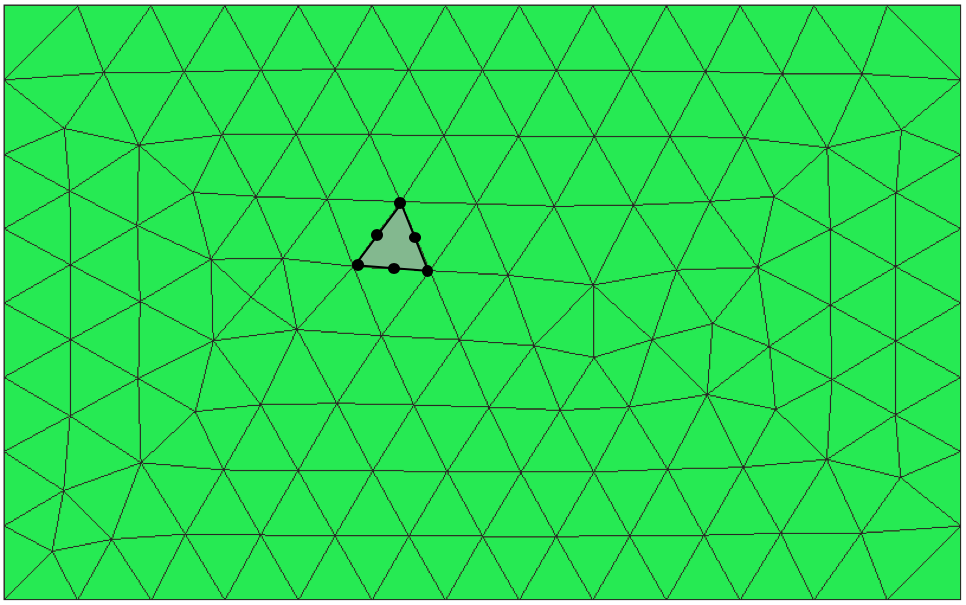
\includegraphics[width=0.45\linewidth]{figs/fe_mesh.png}
\caption{Illustration of a continuous domain discretized into triangular finite elements.}
\label{fig:fe_mesh}
\end{figure}

If \(\psi\) and \(\phi\) are nonzero over the entire domain, every region of the problem is tightly coupled to all other regions, resulting in a dense matrix system. A sparse system can be attained by restricting the shape functions to a nodal basis such that

\beq
\label{eq:Nodal}
\phi_i(\Omega_j)=\delta_{ij}\ ,
\eeq

\noindent where \(\Omega_j\) is the coordinate describing the location of the \(j\)-th node and \(\delta_{ij}\) is the Kronecker delta. The number of nodes in the entire domain, \(N\), determines the number of basis functions used in the approximate solution in Eq.\ \eqref{eq:WRExpansion}. Unless otherwise noted, first-order Lagrange basis functions are used for all solution variables in this work, though the \gls{moose} framework supports higher orders and many other shape function families, such as Hermite and monomial functions.

The boundary terms in Eqs.\ \eqref{eq:PronghornEquations_V2WeakForm}--\eqref{eq:MultiscaleWeak} are integrals over the entire boundary. The boundary may in general be decomposed into the portion on which Dirichelt conditions are specified, \(\Gamma_\text{Dirichlet}\), and the portion on which Neumann conditions are specified, \(\Gamma_\text{Neumann}\). The boundary is the union of these two boundaries

\beq
\Gamma\equiv\Gamma_\text{Dirichlet}\cup\Gamma_\text{Neumann}\ ,
\eeq

\noindent where \(\Gamma_\text{Dirichlet}\cap\Gamma_\text{Neumann}=\emptyset\). On Dirichlet boundaries, the fluxes appearing in the boundary integrals may be unknown. Rather than back-calculating the flux that results in the desired Dirichlet condition on the primal variable, Dirichlet conditions are imposed by requiring

\beq
\psi=0\text{ for }\Gamma\in\Gamma_\text{Dirichlet}\ .
\eeq

\noindent All Dirichlet \glspl{bc} in Pronghorn are strongly enforced. The \texttt{DirichletBC} class, a child of the \texttt{BoundaryCondition} class, abstracts the implementation details of the ``removal'' of Dirichlet nodes from the solve.

\subsection{Method of Lines Time Stepping}
\label{sec:mol}

The expansion used for the approximate solution in Eq.\ \eqref{eq:WRExpansion} is assumed separable in space and time. That is, the expansion coefficients \(C\) are only functions of time, while the basis functions \(\phi\) are only functions of space. All time derivatives in Eqs.\ \eqref{eq:PronghornEquations_V2WeakForm}--\eqref{eq:MultiscaleWeak} are replaced by \gls{fd} approximations, a method that is often referred to as the \gls{mol}. For time step \(n+1\), all other terms in the weak form are evaluated at time \(m\) or time \(m+1\) for explicit and implicit \gls{fd} approximations, respectively.

The \gls{moose} framework abstracts much of the details of the \gls{mol} implementation to \gls{moose} framework classes and the \gls{petsc} library. For instance, there is no time indexing in the variables and material properties referenced in the example source snippets shown in Listings \ref{lst:one} and \ref{lst:two}. Application developers take advantage of polymorphism to represent time derivatives in the source implementation agnostic of the discretization, similar to the spatial representation shown in Section \ref{sec:weak_form}. For example, the source code responsible for residual calculation of the time derivative contribution to Eqs.\ \eqref{eq:MassWeak} and \eqref{eq:Mass2Weak} at a quadrature point is shown in Listing \ref{lst:three}.

\vspace{1em}
\begin{minipage}[c]{0.92\linewidth}
\begin{lstlisting}[caption={Pronghorn source code calculation of \(\int_\Omega\epsilon\frac{\partial\rho_f}{\partial t}\psi d\Omega\).},captionpos=b,label={lst:three}]
Real
MassTimeDerivative::computeQpResidual()
{
  return _epsilon[_qp] * _drho_f_dt[_qp] * _test[_i][_qp];
}
\end{lstlisting}
\end{minipage}

\texttt{MassTimeDerivative} is the kernel class name, \texttt{\_drho\_f\_dt} is the name of the density time derivative \(\partial\rho_f/\partial t\) material coupled to the kernel, and \texttt{\_test} is the name of the weight function \(\psi\). Other terms have the same interpretation as in Listings \ref{lst:one} and \ref{lst:two}. Unless otherwise noted, an implicit Euler discretization is used for all time derivatives in this work.

\subsection[Streamline Upwind Petrov-Galerkin Stabilization]{SUPG Stabilization}
\label{sec:supg}

The continuous \gls{fem} is well-known to be conditionally stable for convection-diffusion equations. Consider the \gls{1d}, linear convection-diffusion equation,

\beq
\label{eq:1DConvectionDiffusion}
-\alpha_d\frac{\partial^2\upsilon}{\partial x^2}+V\frac{\partial \upsilon}{\partial x}=0\ ,
\eeq

\noindent where \(\alpha_d\) is the diffusivity, \(V\) is the velocity, and \(\upsilon\) is a transported scalar. For a linear Lagrange interpolation on uniform elements, the stability criterion for Eq.\ \eqref{eq:1DConvectionDiffusion} is straightforward to derive and is shown in ref. \cite{novak_manual}. This derivation yields

\beq
\label{eq:PeCriterion}
Pe_{el}>1\ ,
\eeq

\noindent where \(Pe_{el}\) is the element Peclet number, defined as

\beq
\label{eq:PeEl}
Pe_{el}\equiv\frac{\|\vec{V}\|h_e}{2\alpha_d}\ ,
\eeq

\noindent where \(h_e\) is the element size. For generality, Eq.\ \eqref{eq:PeEl} is shown in terms of a general diffusivity \(\alpha_d\) rather than the thermal diffusivity \(k/\rho C_p\) used in the definition of \(Pe\) in Eq.\ \eqref{eq:PecletDef}. 

It can be shown that a linear Lagrange interpolation of Eq.\ \eqref{eq:1DConvectionDiffusion} on uniform elements is equivalent to a central \gls{fd} approximation of both the diffusive and convective kernels. This symmetric discretization results in non-physical nodal oscillations for flows with \(Pe_{el}>1\) with magnitudes that tend to increase with \(Pe_{el}\) \cite{novak_manual,zienkiewicz}. 

Fig.\ \ref{fig:Convection_vs_Diffusion} illustrates typical convective and diffusive processes transporting a passive scalar in both space and time between the same \gls{ic} and the same end time. While diffusion is a symmetric phenomenon, convection transports in the direction of velocity such that the flow at a point is only dependent on the upstream conditions. This observation is the underlying cause of the numeric instability\mdash a symmetric discretization of the convective derivative is a poor representation of convective physics unless the symmetry of the diffusive process dominates the upwind nature of convection, or \(Pe_{el}<1\). The same conclusion can be shown in more rigorous manner in terms of the self-adjoint and non-self-adjoint properties of diffusion and convection operators, respectively \cite{zienkiewicz}.

\begin{figure}[!h]
\centering
\begin{subfigure}{.45\textwidth}
  \centering
  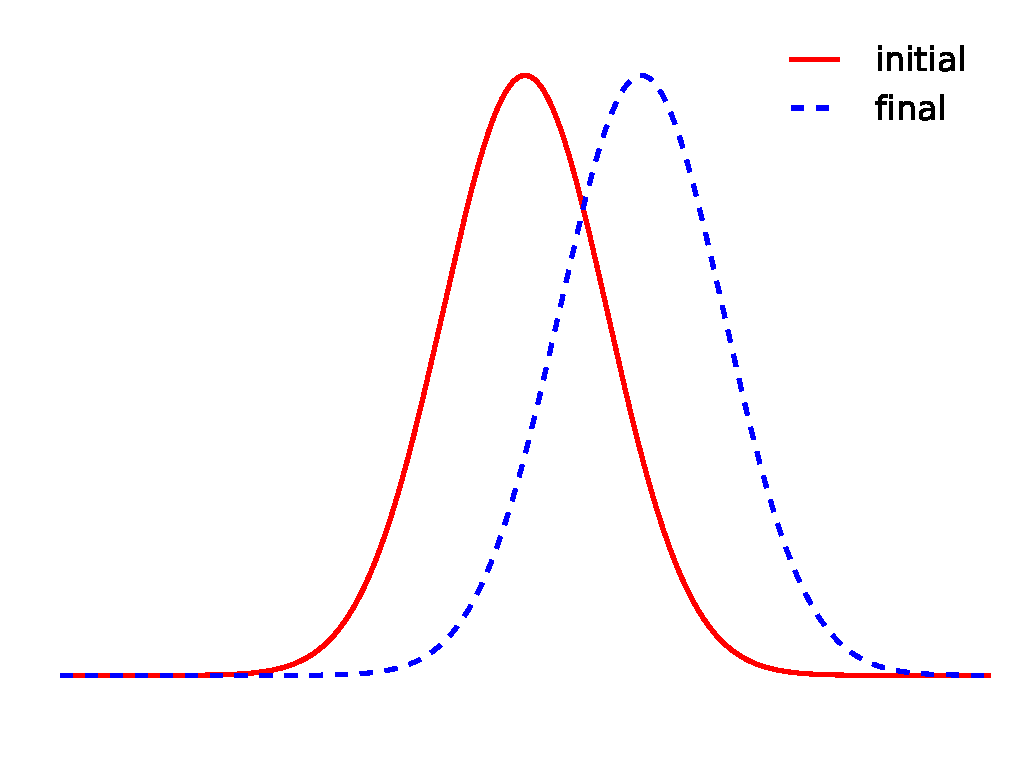
\includegraphics[width=0.9\linewidth]{figs/convective_process.pdf}
  \caption{Convective phenomenon}
\end{subfigure}
\begin{subfigure}{.45\textwidth}
  \centering
  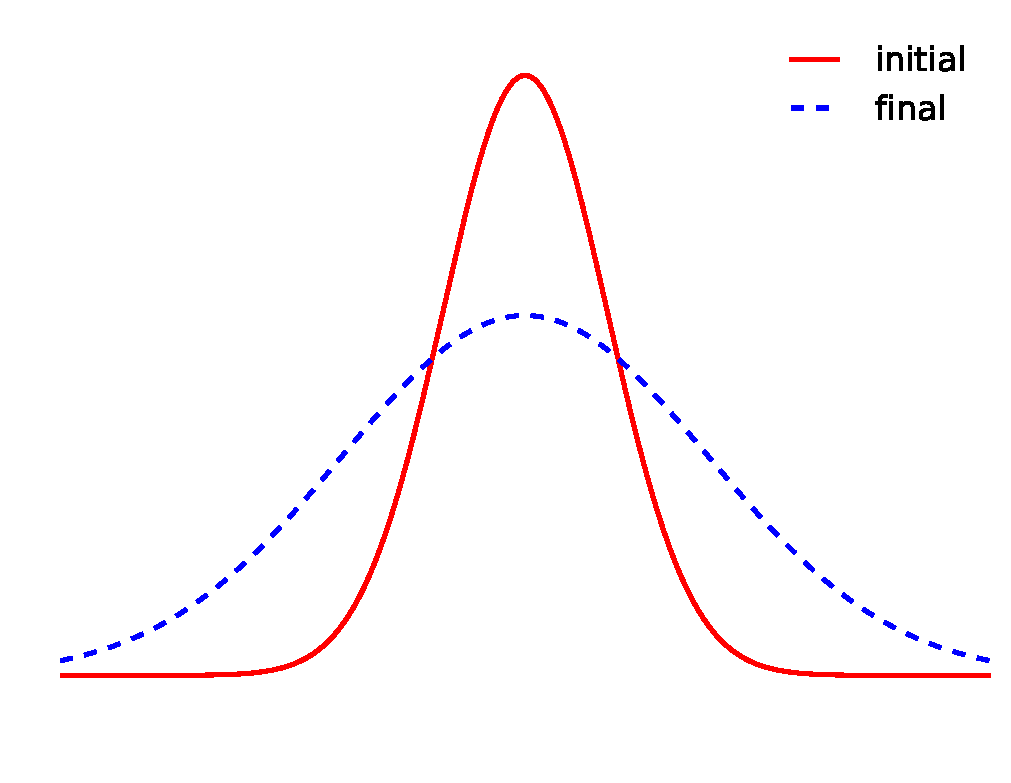
\includegraphics[width=0.9\linewidth]{figs/diffusive_process.pdf}
  \caption{Diffusive phenomenon}
\end{subfigure}
\caption{Difference between (a) convective (flow from left to right) and (b) diffusive transport of a passive scalar from the same \gls{ic} (---) to the same end time (- - -).}
\label{fig:Convection_vs_Diffusion}
\end{figure}

For systems with some diffusion, the mesh can in theory be refined until \(Pe_{el}<1\); however, this strategy is often prohibitively expensive. This section describes an upwind Petrov-Galerkin method that supplements the weak forms in the fluid conservation equations with additional integrals that act to discretize the convective kernels with upwind approximations to better match the directional dependence of convection.

Petrov-Galerkin methods differ from Bubnov-Galerkin methods in that the approximate solution and the weight function no longer live in the same function space; that is, \(\psi\) is no longer given by Eq.\ \eqref{eq:PsiExpansion}. For the Petrov-Galerkin methods considered here, the weight function is instead given as the sum of the original element-continuous weight functions \(\psi\) and an element-discontinuous function \(\psi^\star\),

\beq
\label{eq:pgwf}
\tilde{\psi}=\psi+\psi^\star\ ,
\eeq

\noindent where \(\tilde{\psi}\) represents the Petrov-Galerkin weight function and \(\psi\) is given by Eq.\ \eqref{eq:PsiExpansion}. The weighted residual statement in Eq.\ \eqref{eq:GalerkinInt3} becomes

\beq
\label{eq:PG}
\int_{\Omega}\left\lbrack R\left(C_j\phi_j\right)\right\rbrack^*\phi_i\ d\Omega+\int_{\Omega}\left\lbrack R\left(C_j\phi_j\right)\right\rbrack^*\psi^\star_i\ d\Omega=0\hspace{1cm}\text{for }j\in N\ .
\eeq

\noindent The first integral is the same Bubnov-Galerkin weighted residual statement from Eq.\ \eqref{eq:GalerkinInt3}. While the first integral in Eq.\ \eqref{eq:PG} is integrated by parts where possible, the second integral cannot be integrated by parts because \(\psi^\star\) is discontinuous across elements. If the approximate solution shape functions are sufficiently differentiable to have nonzero and finite derivatives in the second term, the Petrov-Galerkin method is consistent\mdash that is, the solution to Eq.\ \eqref{eq:PG} is the same as the solution to the Bubnov-Galerkin form in Eq.\ \eqref{eq:GalerkinInt3}.

For a linear Lagrange interpolation of Eq.\ \eqref{eq:1DConvectionDiffusion} on uniform elements, selecting \(\psi^\star\) as

\beq
\label{eq:psiStar}
\psi^\star=\frac{h_e}{2\|\vec{V}\|}\vec{V}\cdot\nabla\psi\ 
\eeq

\noindent is equivalent to a central \gls{fd} approximation of the diffusive kernel and an upwind approximation of the convective kernel that eliminates the \(Pe_{el}\) stability criterion \cite{zienkiewicz,brooks,novak_manual}. 

In 1981, Brooks developed a consistent generalization of Eq.\ \eqref{eq:psiStar} to multi-dimensional, coupled, systems of convection-diffusion equations known as the \gls{supg} method that is now widely used in continuous \gls{fem} discretizations of convection-diffusion systems \cite{hauke,tezduyar,kirk,hauke_1998,TH1983,tezduyar1983,zienkiewicz,StabilizationReview}. The remainder of this section describes the application of the \gls{supg} stabilization scheme to the macroscale equations described in Chapter \ref{sec:PhysicalModels}. A detailed discussion of the stabilization is presented to illustrate the extension of the original \gls{supg} method to porous flows. 

The Navier-Stokes and friction-dominated fluid conservation equations are sufficiently different to warrant separate discussions of the \gls{supg} stabilization for each model. Stabilization of the Navier-Stokes model is described first due to its similarity to the conservative forms of convection-diffusion equations for which the \gls{supg} method was originally formulated. Rewrite the fluid conservation equations in the Navier-Stokes model in Eq.\ \eqref{eq:PorousEquations} in compact notation as

\beq
\label{eq:NSConcise}
\frac{\partial(\epsilon\vec{U})}{\partial t}+\frac{\partial(\epsilon\vec{F}_i)}{\partial x_i}-\frac{\partial\vec{G}_i}{\partial x_i}+\vec{S}=\vec{0}\ ,
\eeq

\noindent where \(\vec{U}\) is the vector of conserved quantities,

\beq
\label{eq:EulerNL}
\vec{U}\equiv\begin{bmatrix}\rho_f\\\rho_f V_1\\\rho_f V_2\\\rho_f V_3\\\rho_f E_f
\end{bmatrix}\ ;
\eeq

\noindent \(\vec{F}_i\) is the inviscid flux vector in the \(i\)-th dimension,

\beq
\label{eq:EulerIF}
\vec{F}_i\equiv \begin{bmatrix}\rho_fV_i \\ \rho_f V_1V_i+ P\delta_{1i}\\\rho_f V_2V_i+ P\delta_{2i}\\\rho_f V_3V_i+ P\delta_{3i}\\ \rho_f V_iH_f
\end{bmatrix}\ ;
\eeq

\noindent \(\vec{G}_i\) is the diffusive flux vector in the \(i\)-th dimension,

\beq
\label{eq:PHEquationsConcise}
\vec{G}_i\equiv\begin{bmatrix}0\\\tilde{\mu}\frac{\partial V_1}{\partial x_i}\\\tilde{\mu}\frac{\partial V_2}{\partial x_i}\\\tilde{\mu}\frac{\partial V_3}{\partial x_i}\\ \kappa_f\frac{\partial T_f}{\partial x_i}
\end{bmatrix}\ ;
\eeq

\noindent and \(\vec{S}\) is the source vector,

\beq
\label{eq:EulerS}
\vec{S}=\begin{bmatrix}0\\-\epsilon\rho_fg_1+W\rho_fV_1+P\frac{\partial\epsilon}{\partial x_1}\\-\epsilon\rho_fg_2+W\rho_fV_2+P\frac{\partial\epsilon}{\partial x_2}\\-\epsilon\rho_fg_3+W\rho_fV_3+P\frac{\partial\epsilon}{\partial x_3}\\ -\epsilon\rho_fg_iV_i+\alpha(T_f-T_s)-\dot{q}_f
\end{bmatrix}\ .
\eeq

\noindent For notational simplicity, \(\epsilon\) is shown within the time differentiation term in Eq.\ \eqref{eq:NSConcise} though the actual implementation assumes porosity is independent of time. Define a quasi-linear residual \(\vec{\mathscr{R}}\) as

\beq
\label{eq:StrongResidual}
\vec{\mathscr{R}}\equiv\frac{\partial(\epsilon\vec{U})}{\partial t}+\epsilon\textbf{A}_i\frac{\partial\vec{U}}{\partial x_i}+\vec{F}_i\frac{\partial\epsilon}{\partial x_i}-\frac{\partial \vec{G}_i}{\partial x_i}+\vec{S}\ ,
\eeq

\noindent where \(\textbf{A}_i\) are the inviscid flux Jacobian matrices,

\beq
\label{eq:IFJM}
\textbf{A}_i\equiv\frac{\partial\vec{F}_i}{\partial\vec{U}}\ .
\eeq

\noindent The inviscid flux Jacobian matrices require the partial derivatives of \(P\), \(H_f\), and the components of \(\vec{U}\) with respect to the components of \(\vec{U}\). The partial derivative of \(U_i\) with respect to \(U_j\) is

\beq
\label{eq:UDerivs}
\frac{\partial U_i}{\partial U_j}=\delta_{ij}\ ,
\eeq

\noindent The derivative of \(H_f\) with respect to \(\vec{U}\) is

\beq
\frac{\partial H_f}{\partial \vec{U}}=\frac{1}{\rho_f}\begin{bmatrix}\frac{\partial P}{\partial U_0}-H_f & \frac{\partial P}{\partial U_1} & \frac{\partial P}{\partial U_2} & \frac{\partial P}{\partial U_3} & \frac{\partial P}{\partial U_4}+1\end{bmatrix}\ .
\eeq

\noindent The derivative of pressure with respect to \(\vec{U}\) is written in the form of a chain rule as

\beq
\label{eq:PressureDerivsCons}
\frac{\partial P}{\partial \vec{U}}=\frac{\partial P}{\partial v_f}\frac{\partial v_f}{\partial \vec{U}}+\frac{\partial P}{\partial e_f}\frac{\partial e_f}{\partial \vec{U}}\ ,
\eeq

\noindent where \(v_f\) is the fluid intrinsic phase averaged specific volume; \(\partial P/\partial v_f\) and \(\partial P/\partial e_f\) are obtained from the \gls{eos}; \(\partial v_f/\partial \vec{U}\) is given as

\beq
\label{eq:dvdU}
\frac{\partial v_f}{\partial \vec{U}}=\begin{bmatrix}\frac{1}{\rho_f^2} & 0 & 0 & 0 & 0\end{bmatrix}\ ;
\eeq

\noindent and \(\partial e_f/\partial \vec{U}\) is given as

\beq
\label{eq:dedU}
\frac{\partial e_f}{\partial \vec{U}}=\frac{1}{\rho_f}\begin{bmatrix}\|\vec{V}\|^2-E_f & -V_1 & -V_2 & -V_3 & 1\end{bmatrix}\ .
\eeq

\noindent With the derivatives in Eqs.\ \eqref{eq:UDerivs}--\eqref{eq:dedU}, the inviscid flux Jacobian matrices are

\beq
\label{eq:IFJMi}
\textbf{A}_i=
\begin{bmatrix}
0 & \delta_{1i} & \delta_{2i} & \delta_{3i} & 0\\
\frac{-U_1U_i}{U_0^2}+\delta_{1i}\frac{\partial P}{\partial U_0} & \delta_{1i}\zeta_1+\tilde{\delta}_{1i}\frac{U_i}{U_0} & \delta_{i2}\frac{U_1}{U_0}+\delta_{1i}\frac{\partial P}{\partial U_2} & \delta_{i3}\frac{U_1}{U_0}+\delta_{1i}\frac{\partial P}{\partial U_3} & \delta_{1i}\frac{\partial P}{\partial U_4}\\
\frac{-U_2U_i}{U_0^2}+\delta_{2i}\frac{\partial P}{\partial U_0} & \delta_{1i}\frac{U_2}{U_0}+\delta_{2i}\frac{\partial P}{\partial U_1} & \delta_{2i}\zeta_2+\tilde{\delta}_{2i}\frac{U_i}{U_0} & \delta_{i3}\frac{U_2}{U_0}+\delta_{2i}\frac{\partial P}{\partial U_3} & \delta_{2i}\frac{\partial P}{\partial U_4}\\
\frac{-U_3U_i}{U_0^2}+\delta_{3i}\frac{\partial P}{\partial U_0} & \delta_{1i}\frac{U_3}{U_0}+\delta_{3i}\frac{\partial P}{\partial U_1} & \delta_{2i}\frac{U_3}{U_0}+\delta_{3i}\frac{\partial P}{\partial U_2} & \delta_{3i}\zeta_3+\tilde{\delta}_{3i}\frac{U_i}{U_0} & \delta_{3i}\frac{\partial P}{\partial U_4}\\
U_i\frac{\partial H_f}{\partial U_0} & U_i\frac{\partial H_f}{\partial U_1}+\delta_{1i}H_f & U_i\frac{\partial H_f}{\partial U_2}+\delta_{2i}H_f & U_i\frac{\partial H_f}{\partial U_3}+\delta_{3i}H_f & U_i\frac{\partial H_f}{\partial U_4}\\
\end{bmatrix}\ ,
\eeq

\noindent where the following terms are defined for conciseness,

\beq
\label{eq:tilde_delta}
\tilde{\delta}_{ij}\equiv1-\delta_{ij}\ ,
\eeq

\beq
\label{eq:zeta_placeholder}
\zeta_i\equiv\frac{2U_i}{U_0}+\frac{\partial P}{\partial U_i}\ .
\eeq

\noindent All prerequisite notation has been introduced to now describe the stabilization. The \gls{supg} method adds the following integral to the Bubnov-Galerkin weak form,

\beq
\label{eq:supg1}
\int_\Omega\epsilon\left\lbrack\textbf{A}_i\left(\tau_{SUPG}\ \vec{\mathscr{R}}\right)\right\rbrack\cdot\frac{\partial\vec{W}}{\partial x_i}d\Omega\ ,
\eeq

\noindent where \(\tau_{SUPG}\) is a matrix of stabilization coefficients and \(\vec{W}\) is the vector of weight functions corresponding to each coupled equation. To clearly illustrate the indexing, rewrite Eq.\ \eqref{eq:supg1} as

\beq
\label{eq:supg2}
\int_\Omega\epsilon\textbf{A}_{i,jk\ }\tau_{SUPG,kl\ }\mathscr{R}_l\frac{\partial W_j}{\partial x_i}d\Omega\ .
\eeq

\noindent For the five coupled equations in Eq.\ \eqref{eq:NSConcise} in three spatial dimensions, \(j\), \(k\), \(l=1,2,3,4,5\) and \(i=1,2,3\). In other words, \(j\), \(k\), \(l\) represent the number of coupled equations and \(i\) represents the number of spatial dimensions. The weak form of the Navier-Stokes model with the \gls{supg} stabilization is then

\beqa
\label{eq:EqnWeakForm}
\int_{\Omega}\left\lbrack\epsilon\vec{W}\cdot\frac{\partial\vec{U}}{\partial t}+\frac{\partial\vec{W}}{\partial x_i}\cdot\left(\vec{G}_i-\epsilon\vec{F}_i\right)+\vec{W}\cdot\vec{S}\right\rbrack d\Omega+\int_{\Gamma}\left(\epsilon\vec{F}_i-\vec{G}_i\right)\cdot\vec{W}n_id\Gamma\ +\hspace{1cm}\\
\int_\Omega\epsilon\left\lbrack\textbf{A}_i\left(\tau_{SUPG}\ \vec{\mathscr{R}}\right)\right\rbrack\cdot\frac{\partial\vec{W}}{\partial x_i}d\Omega=0\ ,
\eeqa

\noindent where integration by parts is applied only to the element-continuous terms. The first two integrals in Eq.\ \eqref{eq:EqnWeakForm} have already been presented in Eq.\ \eqref{eq:PronghornEquations_V2WeakForm}.

While perhaps not immediately apparent, Eq.\ \eqref{eq:supg1} is equivalent to upwinding in directions parallel to the velocity vector. To the \(j\)-th coupled equation is added an integral involving terms proportional to \(\vec{V}\cdot\nabla W_j\), \(\vec{\mathscr{R}}_u\cdot\nabla W_j\), and \(\partial W_j/\partial x_j\) (no summation implied), where \(\vec{\mathscr{R}}_u\) is the vector of momentum quasi-linear strong residuals. These new terms have a clear resemblance to the \gls{1d} \(\psi^\star\) in Eq.\ \eqref{eq:psiStar} that introduced an upwind discretization of the convective derivative, but now generalized to coupled systems of equations. As an instructive example, Appendix \ref{sec:supg_app} shows the \gls{supg} integrals in Eq.\ \eqref{eq:EqnWeakForm} for the mass, momentum, and energy conservation equations in the Navier-Stokes model with the ideal gas \gls{eos}.

The friction-dominated model lacks convective terms in the momentum conservation equations and the fluid energy conservation equation is not written in conservative form. Rather than cast the friction-dominated model into the notation in Eq.\ \eqref{eq:NSConcise}, carrying through the algebra in Eq.\ \eqref{eq:supg1} shows that a term proportional to \(\vec{\mathscr{R}}_i\cdot\nabla W_0\) is added to the Navier-Stokes mass conservation equation. Extending this concept to the friction-dominated model, the following integral is added to the friction-dominated mass conservation equation,

\beq
\label{eq:fd1}
\int_\Omega \tilde{\tau}\left(\epsilon\nabla P-\epsilon\rho_f\vec{g}+W\rho_f\vec{V}\right)\cdot\nabla\psi d\Omega\ ,
\eeq

\noindent where \(\tilde{\tau}\) is a scalar stabilization parameter. The weak form of the friction-dominated mass conservation equation with the \gls{supg} stabilization is then

\beqa
\label{eq:qqq1}
\int_\Omega\epsilon\frac{\partial\rho_f}{\partial t}\psi d\Omega-\int_\Omega\left\lbrack\frac{\epsilon^2}{W}\left(\rho_f\vec{g}-\nabla P\right)\right\rbrack\cdot\nabla\psi d\Omega+\int_\Gamma\left\lbrack\frac{\epsilon^2}{W}\left(\rho_f\vec{g}-\nabla P\right)\right\rbrack \psi d\Gamma+\hspace{1cm}\\
\int_\Omega \tilde{\tau}\left(\epsilon\nabla P-\epsilon\rho_f\vec{g}+W\rho_f\vec{V}\right)\cdot\nabla\psi d\Omega=0\ .
\eeqa

\noindent The first two integrals in Eq.\ \eqref{eq:qqq1} have already been presented in Eq.\ \eqref{eq:Mass2Weak}. No additional integrals are added to the momentum conservation equations due to the lack of convective terms. 

Finally, the fluid energy conservation equation is stabilized using the single-equation form suggested by Eq.\ \eqref{eq:psiStar} by adding the following integral to the fluid energy conservation equation,

\beq
\label{eq:fd2}
\int_\Omega\tilde{\tau}\left\lbrack\epsilon\rho_fC_{p,f}\frac{\partial T_f}{\partial t}+\epsilon\rho_fC_{p,f}\vec{V}\cdot\nabla T_f-\nabla\cdot(\kappa_f\nabla T_f)+\alpha(T_f-T_s)-\dot{q}_f\right\rbrack\vec{V}\cdot\nabla \psi d\Omega\ .
\eeq

\noindent The weak form of the friction-dominated fluid energy conservation equation with the \gls{supg} stabilization is then

\beqa
\label{eq:qqq2}
\int_\Omega\left\lbrack\epsilon\rho_fC_{p,f}\frac{\partial T_f}{\partial t}+\epsilon\rho_fC_{p,f}\vec{V}\cdot\nabla T_f+\alpha(T_f-T_s)-\dot{q}_f\right\rbrack\psi d\Omega+\int_\Omega\kappa_f\nabla T_f\cdot\nabla \psi d\Omega\ +\hspace{0.3cm}\\
\int_\Gamma\kappa_f\nabla T_f\cdot\hat{n}\psi d\Gamma+\int_\Omega\tilde{\tau}\left(\epsilon\rho_fC_{p,f}\frac{\partial T_f}{\partial t}+\epsilon\rho_fC_{p,f}\vec{V}\cdot\nabla T_f\right)\vec{V}\cdot\nabla\psi d\Omega\ +\hspace{0.15cm}\\
\int_\Omega\tilde{\tau}\left\lbrack-\nabla\cdot(\kappa_f\nabla T_f)+\alpha(T_f-T_s)-\dot{q}_f\right\rbrack\vec{V}\cdot\nabla \psi d\Omega=0\ .
\eeqa

\noindent The first two integrals in Eq.\ \eqref{eq:qqq2} have already been presented in Eq.\ \eqref{eq:Energy2Weak}. The \gls{supg} stabilization terms in Eq.\ \eqref{eq:supg1} for the Navier-Stokes model and Eqs.\ \eqref{eq:fd1} and \eqref{eq:fd2} for the friction-dominated model are implemented in Pronghorn in a similar manner as the other kernels as described in Section \ref{sec:weak_form}. 

\(\tau_{SUPG}\) represents a matrix of intrinsic time scales; for coupled systems of equations, each component in \(\tau_{SUPG}\) is a combination of the waves associated with the eigenvalues of the equation system. Rather than solve an eigenvalue problem at each quadrature point, computational efficiency motivates a diagonal approximation,

\beq
\label{eq:tauSUPG}
\tau_{SUPG}=\begin{bmatrix}
\tau_c & 0 & 0 & 0 & 0\\
0 & \tau_{u} & 0 & 0 & 0\\
0 & 0 & \tau_{u} & 0 & 0\\
0 & 0 & 0 & \tau_{u} & 0\\
0 & 0 & 0 & 0 & \tau_e\\
\end{bmatrix}\ ,
\eeq

\noindent where the stabilization parameters for the mass, momentum, and energy conservation equations are \(\tau_c\), \(\tau_u\), and \(\tau_e\), respectively \cite{hauke,tezduyar,hauke_1998,kirk,TH1983,tezduyar1983}. \(\tau_c\), \(\tau_u\), and \(\tau_e\) are typically selected as characteristic time scales representing normalized temporal, advective, and diffusive terms in the weak form \cite{tezduyar}. 

Three different time scales are considered in the construction of \(\tau_c\), \(\tau_u\), and \(\tau_e\)\mdash 1)~a transient limit, \(\tau_\text{temporal}\); 2)~an advective limit, \(\tau_\text{advective}\); and 3)~a diffusive limit, \(\tau_\text{diffusive}\). These time scales are combined into a single representative time scale with smooth transitions among its components,

\beq
\label{eq:switchTau}
\tau_j=\left\lbrack\left(\frac{1}{\tau_\text{temporal}}\right)^2+\left(\frac{1}{\tau_\text{advective}}\right)^2+\left(\frac{1}{\tau_\text{diffusive}}\right)^2\right\rbrack^{-1/2}\ ,
\eeq

\noindent where \(j=c\), \(u\), \(e\). The \(\tau_\text{temporal}\), \(\tau_\text{advective}\), and \(\tau_\text{diffusive}\) terms may in general be unique for each of the conservation equations. However, for the present analysis, the mass, momentum, and energy conservation equations share the same advective and temporal limits. The advective limit is given as

\beq
\label{eq:tau1}
\tau_\text{advective}=\frac{h_e}{2\left(\|\vec{V}\|+c\right)}\ ,
\eeq

\noindent and the temporal limit is given as

\beq
\label{eq:tau2}
\tau_\text{temporal}=\frac{\Delta t}{2}\ .
\eeq

\noindent Lacking diffusive terms, there is no diffusive limit for the mass conservation equation. For the momentum conservation equation, the diffusive limit is given as

\beq
\label{eq:tau3}
\tau_\text{diffusive}=\frac{\rho_fh_e^2}{4\left(\tilde{\mu}/\epsilon\right)}\ ,
\eeq

\noindent while for the energy conservation equation is given as

\beq
\label{eq:tau4}
\tau_\text{diffusive}=\frac{\rho_fC_{p,f}h_e^2}{4\left(\kappa_f/\epsilon\right)}\ .
\eeq

\noindent The scalar stabilization parameter \(\tilde{\tau}\) in the \gls{supg} stabilization of the friction-dominated model is taken as Eq.\ \eqref{eq:tau4}. The element size \(h_e\) is for simplicity taken as the minimum dimension of the element, though methods based on flow-aligned or element-averaged scales have been used elsewhere \cite{hauke_1998,hauke,tezduyar1983,tezduyar}. 

The selection of \(\tau_{SUPG}\) requires a balance between accuracy and stability\mdash too small a \(\tau_{SUPG}\) will still exhibit nodal oscillations, while too large a \(\tau_{SUPG}\) will result in excessive diffusion for basis functions with orders less than the highest derivative in the strong form \gls{pde}. The above definitions for \(\tau_c\), \(\tau_u\), and \(\tau_e\) are only approximate, and a multiplier \(\tilde{C}\) is used to scale the stabilization parameter. All simulations should be run for a number of \(\tilde{C}\) values to determine an appropriate balance between stability and accuracy. \

\section{Solution Methods}
\label{sec:solution}
This section describes the numerical solution of the coupled system of macroscale, mesoscale, and microscale equations. A Picard iteration described in Section \ref{sec:multiscale_solution} is used to couple the solutions on the three length scales, where the solution on each individual scale is obtained with a Newton-Krylov method described in Section \ref{sec:nonlinear}.

\subsection{Picard Iteration of Multiple Applications}
\label{sec:multiscale_solution}

Coupling between the macro, meso, and micro length scales is achieved using Picard iteration. The \gls{moose} framework uses a hierarchical tree-like system to control execution of and data transfer between multiple applications within a single simulation. A ``master'' application controls a number of sub-applications and facilitates data transfer between itself and the sub-applications. Each sub-application may itself control a number of sub-applications, locally acting as a master application to sub-applications double nested relative to the top-level application. 

The coupling tree is highly parallelized. The master application uses all processors, while all its sub-applications run simultaneously in parallel with the resources allocated to the local master application. For instance, consider a three-tiered coupling system with application \(\mathcal{A}\) controlling five sub-applications \(\mathcal{B}_i\) for \(i=1\cdots 5\), each of which controls two sub-applications \(\mathcal{C}_{ij}\) for \(j=1, 2\). Allocating a total of 60 \gls{mpi} processes to application \(\mathcal{A}\) will run each of the \(\mathcal{B}\) applications with 12 processes and each of the \(\mathcal{C}\) applications with 6 processes; all \(\mathcal{B}\) processes run in parallel with one another and all \(\mathcal{C}\) processes run in parallel with one another. 

\gls{moose}'s coupling system specifically aims to address many of the shortcomings of earlier multiphysics simulations that relied on rigid one-to-one spatial and temporal data transfers through the file system. All \gls{moose} applications may be coupled on different spatial meshes with subcycling time stepping, and all data is communicated in memory. 
% TODO - could cite multiphysics papers here

As an example, Fig.\ \ref{fig:multiapp} illustrates one possible execution and communication structure within a single Picard iteration for a simulation involving two applications on the same spatial domain. Both the master application and sub-application may in general solve a set of coupled nonlinear equations. In Picard iteration \(n\) within the time step incrementing to simulation time \(t\), the master application first solves a set of coupled equations with the Newton-Krylov method described in Section \ref{sec:nonlinear}. The master application then transfers the variable \(T\) to a sub-application that depends on that variable, such as through a source term or material property. Interpolation between meshes, sampling from element centroids, and functional expansions are several of the mechanisms available for representing data transfers between applications. For this example, Fig.\ \ref{fig:multiapp} depicts this data transfer as a mesh interpolation. Next, the sub-application solves a set of coupled equations with the Newton-Krylov method described in Section \ref{sec:nonlinear}. The master application then retrieves the variable \(\phi\) from the sub-application to use in dependent terms in its set of equations. The coupled simulation is converged and proceeds to the next time step if the relative change in the solution from the previous Picard iteration is less than a specified tolerance. If not converged, the Picard iteration is repeated. The example illustrated in Fig.\ \ref{fig:multiapp} is fairly simplistic, and the multi-application execution and data transfer system in \gls{moose} accommodates many other types of coupling, such as scalar and boundary coupling, with more fine-grained communication patterns. 

\begin{figure}[!h]
\centering
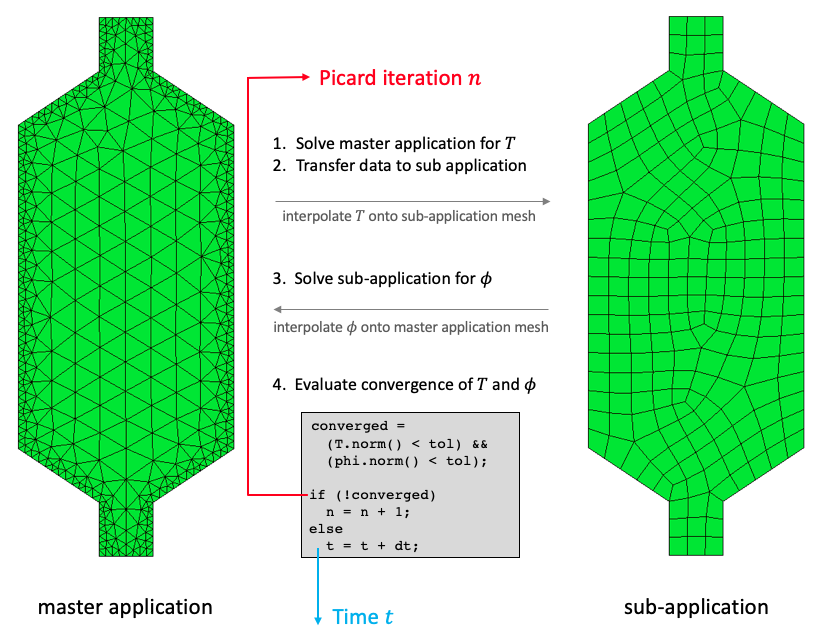
\includegraphics[width=0.9\linewidth]{figs/multiapp.png}
\caption{Illustration of one possible execution and communication structure for coupling multiple applications within the \gls{moose} framework.}
\label{fig:multiapp}
\end{figure}

Fig.\ \ref{fig:multiscale_pbr} shows an illustration of the length scale coupling in Pronghorn when the \gls{hsd} is used to describe the internal pebble heat transfer. The macroscale model is the master application, which controls the execution of the ``first-tier'' mesoscale sub-applications. Each mesoscale application controls the execution of the ``second-tier'' microscale sub-applications. In a single Picard iteration, the multiscale coupling procedure with the \gls{hsd} meso and micro scale model is as follows\mdash

\begin{enumerate}
\itemsep0.3em
\item The master application solves the macroscale model.
\item The master application calculates the average solid surface temperature \(T_s\) and solid power density in each element of the macroscale mesh.
\item The master application transfers the averaged solid surface temperature as a \gls{bc} and the averaged solid power density as a source term to a mesoscale sub-application in each element. Six macroscale elements are highlighted in Fig.\ \ref{fig:multiscale_pbr}; the ``color'' in the element represents the magnitude of the solid surface temperature used as a \gls{bc} in the mesoscale model. Note the similarity of this process to that illustrated in Fig.\ \ref{fig:meso}.
\item The first-tier sub-applications solve the mesoscale models, which themselves consist of several steps repeated until convergence of the pebble temperature distribution\mdash
	\begin{enumerate}
  \itemsep0.3em
	\item The first-tier sub-applications solve the mesoscale model given a previous microscale solution in each element of the mesoscale mesh.
	\item The first-tier sub-applications calculate averaged power densities in each element of the mesoscale mesh.
	\item The first-tier sub-applications transfer the averaged power densities as a source term to a microscale sub-application in each element.
	\item The second-tier sub-applications solve the microscale models.
	\item The first-tier sub-applications retrieve the microscale solution in each element of the mesoscale mesh and apply the continuity in heat flux and temperature \gls{bc} with the summation in Eq.\ \eqref{eq:MultiscaleSolution}.
	\end{enumerate}
\end{enumerate}

\begin{figure}[!h]
\centering
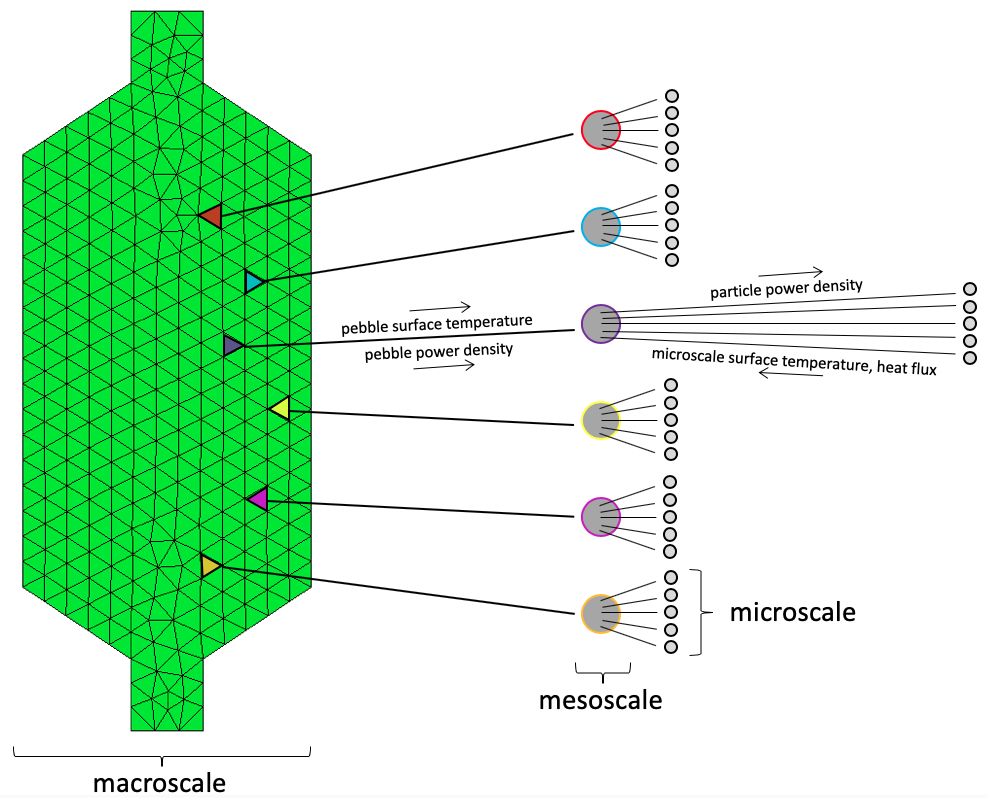
\includegraphics[width=0.8\linewidth]{figs/multiscale_pbr_d.png}
\caption{Illustration of the hierarchical multiscale execution and data transfer in Pronghorn when using the \gls{hsd} pebble model.}
\label{fig:multiscale_pbr}
\end{figure}

It is important to note that this coupling algorithm only applies to steady-state flows. An extension to transient modeling requires communication of the pebble surface heat flux to the macroscale application for use as a source term in the fluid energy conservation equation instead of the \(\alpha(T_f-T_s)\) kernel, eliminating the macroscale solid energy conservation equation. Transient capabilities are to be implemented in the near future. 

For generality, Fig.\ \ref{fig:multiscale_pbr} shows a number of microscale simulations in each pebble. As discussed in Section \ref{sec:mesomicro}, the thin fuel-matrix region of the \gls{pbfhr} modeled in Chapter \ref{sec:pbfhr} warrants the simplifying assumption that a single average microscale domain in each pebble captures the average particle heat transfer. Therefore, a single microscale domain is simulated in each mesoscale domain.

As compared to the \gls{hsd} model, the multiscale coupling procedure is much simpler for the \gls{hl} model due to the use of a single differential equation to describe the pebble temperature distribution. For the \gls{hl} method, the above calculation sequence replaces step 4, and all its sub-steps, with solution of the \gls{hl} model in Eq.\ \eqref{eq:oem} in a first-tier sub-application. The \gls{hl} method therefore does not involve second-tier sub-applications. 

\subsection{Newton-Krylov Nonlinear Solution}
\label{sec:nonlinear}

This section describes the solution of a nonlinear system of equations\mdash for the macroscale model, this refers to the four coupled equations in Eq.\ \eqref{eq:PorousEquations} or \eqref{eq:PrimitiveEqns}; for the mesoscale, this refers to the \gls{hl} model in Eq.\ \eqref{eq:oem} or the \gls{hsd} model in \eqref{eq:MesoscaleSolution}; and for the microscale, this refers to the \gls{hsd} model in Eq.\ \eqref{eq:MicroscaleSolution}. Notably, Pronghorn differs from many Navier-Stokes solvers in that the fluid conservation equations are solved together in the same matrix system, rather than with segregated solvers such as \gls{simple}.

A Newton-Krylov method is used to solve the \gls{fe} discretized forms of the multiscale models presented in Section \ref{sec:weak_form} with the \gls{supg} stabilization terms given in Section \ref{sec:supg}. The nonlinear system of equations is a root-finding problem; extending Eq.\ \eqref{eq:residual} to the discretized case, this nonlinear system is

\beq
\label{eq:nonlinear2}
\vec{R}(\vec{u})=0\ ,
\eeq

\noindent where \(\vec{R}\) is the discrete nonlinear residual vector and \(\vec{u}\) is the discrete approximate nonlinear solution. A Newton-Krylov method first linearizes Eq.\ \eqref{eq:nonlinear2} to the form

\beq
\label{eq:linear}
\textbf{A}\vec{x}=\vec{b}\ ,
\eeq

\noindent where \(\textbf{A}\) is a matrix, \(\vec{x}\) is the linear solution vector, and \(\vec{b}\) is the \gls{rhs} vector; linearization with Newton's method is explained shortly. Following this linearization, the Newton-Krylov method involves two main loops\mdash 1)~an inner loop with index \(k\) that iteratively solves for \(\vec{x}\) in Eq.\ \eqref{eq:linear}; and 2)~an outer loop with index \(i\) that iteratively solves for \(\vec{u}\) in Eq.\ \eqref{eq:nonlinear2}.

Linearization is performed with Newton's method by forming a Taylor series approximation about the current nonlinear iterate,

\beq
\label{eq:TaylorSeriesResidual}
\vec{R}(\vec{u}_{i+1})=\vec{R}(\vec{u}_i)+\frac{\partial\vec{R}(\vec{u}_i)}{\partial \vec{u}}(\vec{u}_{i+1}-\vec{u}_i)+\mathcal{O}(\vec{u}_{i+1}-\vec{u}_i)^2\ .
\eeq

\noindent Setting Eq.\ \eqref{eq:TaylorSeriesResidual} to zero and neglecting higher-order terms, a linear form is obtained,

\beq
\label{eq:linear3}
\textbf{J}(\vec{u}_i)\vec{\delta}_i=-\vec{R}(\vec{u}_i)\ ,
\eeq

\noindent where \(\textbf{J}(\vec{u}_i)\) is the Jacobian of the \(i\)-th iterate, defined as

\beq
\label{eq:JacobianDef}
\textbf{J}(\vec{u}_i)\equiv\frac{\partial \vec{R}(\vec{u}_i)}{\partial\vec{u}}\ ,
\eeq

\noindent and \(\vec{\delta}_i\) is the update vector, defined as

\beq
\label{eq:update}
\vec{\delta}_i\equiv\vec{u}_{i+1}-\vec{u}_i\ .
\eeq

\noindent Comparing Eq.\ \eqref{eq:linear3} with the general linear form in Eq.\ \eqref{eq:linear} shows that \textbf{A} represents \(\textbf{J}\), \(\vec{b}\) represents \(-\vec{R}\), and \(\vec{x}\) represents \(\vec{\delta}_i\). To match the convention used in most linear algebra texts, the notation in Eq.\ \eqref{eq:linear} is used in the remainder of this section to describe the linear problem in Eq.\ \eqref{eq:linear3}.

To summarize the Newton-Krylov method, the inner loop iteratively solves for \(\vec{x}_k\) until the norm of the linear residual in the \(k\)-th iteration, \(\vec{r}_k\), is less than a specified tolerance \(\varepsilon_l\),

\beq
\label{eq:convergence_linear}
\|\vec{r}_k\|\leq\varepsilon_l\ ,
\eeq 

\noindent where

\beq
\label{eq:linear_residual}
\vec{r}_k\equiv\textbf{A}\vec{x}_k-\vec{b}\ .
\eeq

\noindent After the linear iterations have converged, the \((i+1)\)-th nonlinear iterate is calculated as

\beq
\vec{u}_{i+1}=\vec{u}_i+\vec{x}_k\ .
\eeq

\noindent The matrix \(\textbf{A}\) and \gls{rhs} vector \(\vec{b}\) are then updated based on \(\vec{u}_{i+1}\), and the process repeated to obtain the next nonlinear iterate \(\vec{u}_{i+2}\). 

The nonlinear problem is converged once the norm of the nonlinear residual in the \(i\)-th iteration is less than a specified tolerance \(\varepsilon_n\),

\beq
\|\vec{R}(\vec{u}_i)\|\leq\varepsilon_n\ .
\eeq

\noindent The \gls{gmres} method, a Krylov subspace iterative method commonly used to solve non-symmetric linear systems, is used for solution of Eq.\ \eqref{eq:linear} \cite{saad}. A Krylov space is a vector space built by repeatedly applying a matrix to a vector. The Krylov space \(\mathcal{K}_k\) built by repeatedly applying \(\textbf{A}\) to \(\vec{r}_0\) is

\begin{equation}
\label{eq:krylov_space}
\mathcal{K}_k=\textrm{span}\{\vec{r}_0, \textbf{A}\vec{r}_0, \cdots, \textbf{A}^{k-1}\vec{r}_0\}\ .
\end{equation}

\noindent In each linear iteration, the \gls{gmres} method computes the \((k+1)\)-th linear iterate from the space \(\vec{x}_0+\mathcal{K}_k\) by minimizing the L$^2$ norm of the linear residual over \(\vec{x}_0+\mathcal{K}_k\). 

The convergence of iterative linear solvers such as \gls{gmres} generally depends on the condition number and location and clustering of the eigenvalues of \textbf{A} \cite{trefethen}. The total number of linear iterations can be dramatically reduced by preconditioning the linear system, or applying a preconditioner matrix \textbf{M} in such a way as to reduce the condition number and/or shift the eigenvalue spectrum \cite{benzi}. \gls{gmres} and other linear solvers based on minimizing residuals typically employ a ``right'' preconditioning process, which applies \textbf{M} to the linear system in Eq.\ \eqref{eq:linear} as

\beq
\textbf{A}\textbf{M}^{-1}(\textbf{M}\vec{x})=\vec{b}\ ,
\eeq

\noindent so that the residual is unchanged. \gls{petsc} options are exposed directly to \gls{moose} applications, enabling the use of a large set of preconditioners \cite{petsc}. Preconditioner selection is often problem-specific, but an \gls{asm} \gls{smp} with \gls{ilu} on sub-blocks is often sufficient.

\gls{ad}, sometimes referred to as ``algorithmic differentiation,'' is used to calculate the Jacobians in Eq.\ \eqref{eq:JacobianDef} \cite{ad}. Operator overloads are defined for all of the fundamental arithmetic operators, such as addition, subtraction, multiplication, and division, as well as for elementary functions such as exponentials and logarithms. These overloads then systematically apply the chain rule to the sequence of arithmetic operations used to construct the residual \(\vec{R}\) to compute a working precision accurate estimate of the derivatives of \(\vec{R}\) with respect to \(\vec{u}\). The use of \gls{ad} enables faster application development by avoiding the by-hand derivation of nonlinear residual derivatives. In many cases, \gls{ad} also decreases the number of linear and nonlinear iterations due to the more accurate Jacobian evaluation. The use of \gls{ad} also allows seamless interchange between different sets of solution variables without any modifications to the kernel and \gls{bc} classes that would otherwise be required for by-hand Jacobian evaluation.

\section{Software Engineering Design}
\label{sec:software}
% TODO: change many to all?

High-quality software is essential to support the safety analysis of nuclear reactors. The \gls{moose} framework meets many \gls{nqa1} standards that certify software providing safety functions for nuclear facilities. The \gls{moose} framework meets these standards through supporting a software engineering design incorporating the use of git version control, GitHub pull requests and peer review, \gls{ci} with regression and unit tests of the framework and registered applications, and code style and formatting requirements \cite{slaughter}. Pronghorn shares many of these software engineering best practices, including\mdash

\begin{itemize}
\itemsep0.3em
\item \gls{inl} GitLab repository with issue tracking and peer review of all proposed changes;
\item \gls{ci} with a regression and Googletest unit test suite to ensure proper application behavior before new feature addition to both Pronghorn and the \gls{moose} framework;
\item Hierarchical \gls{xml} input file syntax;
\item In-source \texttt{C++} Doxygen documentation;
\item In-source Markdown for rendering a navigable user guide as a \gls{html} web page; and
\item In-repository theory manual.
\end{itemize}

Select examples from Pronghorn's regression and unit test suite are described at greater length in Chapter \ref{sec:vv}.
